The top quark induced background in the \WW\ analysis originates from
\ttbar and the single top (\tw) processes, the latter being especially imporatant 
in the 0-Jet bin.
A consistent theoretical description of the two processes at high perturbation
orders is not straightforward to attain as already at NLO some \tw diagrams
coincides with LO $\ttbar$ ones \cite{singleTopInterference}.
The Monte Carlo simulated samples used in the analysis exploit an approach
recently proposed \cite{singleTopRemoval}, which addresses the overlap by discarding
the common diagrams from the \tw process either at amplitude level 
({\it Diagram Removal}) or at cross section level ({\it Diagram Subtraction}).
The former is considered the default scheme, whereas the latter is used
as cross check.

The procedure to estimate the top background from data in the case of the 0-Jet bin
established in \cite{HWW2011} has been adapted to the new theoretical description of \ttbar and \tw.
Before assessing the adjustments to the procedure, it is worth reviewing the key points of
the normalization strategy. 

Rejection for the top background is achieved by top-tagged events, i.e. events with a b-tagged jet
or a soft muon as defined in Section~\ref{sec:sel_toptag}. 
The estimation of this background relies on the measurement on data of the top-tagging efficiency.
The procedure deployed in \cite{HWW2011} in the case of the 0-Jet bin proceeds accordingly to the following steps:
\begin{enumerate}
\item A top enriched region is defined requiring exactly one b-tagged jet with \pt larger than $30$ GeV (denumerator). 
Those events among this sample with at least one b-tagged jets with $7<\ensuremath{p_\mathrm{T}}<30$ GeV 
or one soft muon defines the numerator. The ratio of the yields in the numerator and denumerator properly corrected
from other backgrounds contamination provides the top-tagging efficiency 
for one ``top-taggable'' leg, $\epsilon_{1leg}^{data}$. 
\item The actual top-tagging efficiency, $\epsilon_{topTag}^{data}$, is computed accounting for 
the \ttbar fraction of the top background ($f_{t\bar{t}}^{MC}$) accordingly to the formula:
\begin{equation} \label{eq:oldTopTagEff}
\epsilon_{topTag}^{data} = f_{t\bar{t}}^{MC}(1-(1-\epsilon_{1leg}^{data})^2) + (1-f_{t\bar{t}}^{MC})\epsilon_{1leg}^{data}
\end{equation} 
where the first term on the right accounts for \ttbar (two taggable legs) and the second term for \tw 
(one taggable leg). The value $f_{t\bar{t}}^{MC}$ is determined from Monte Carlo in the 0-Jet bin 
at the \WW preselection level, removing the anti top-tagging.
\item A dedicated control region is defined in the 0-Jet bin by requiring top-tagged events. 
The data yields in this region corrected for the other backgrounds contaminations are then used
together with top-tagging efficiency to predict the top background after \WW preselections level:
\begin{equation} \label{eq:topExtrapolation}
N^{top}_{WW region}=N_{topTag}^{top}\frac{1-\epsilon_{topTag}^{data}}{\epsilon_{topTag}^{data}} = 
(N_{topTag}^{data}-N_{other-bkg}^{data})\frac{1-\epsilon_{topTag}^{data}}{\epsilon_{topTag}^{data}}
\end{equation} 
\end{enumerate} 

The top background is estimated at the \WW preselections level where a common scale factor 
for the Monte Carlo \ttbar and \tw samples is computed. 
Once properly normalized, those samples are used either to predict
the correspoding yields after the mass dependent Higgs selections for the cut based analysis 
(Section \ref{sec:anal_cutbased}), or as templates for the multivariate analysis.

In a nutshell, the new procedure refines the way the top-tagging efficiency is extracted from data,
taking properly into account the different features of \ttbar and \tw.
\begin{itemize}

\item The top-tagging efficiency for one leg, $\epsilon_{1leg}^{data}$, is computed for \ttbar only, 
that is both non-top backgrounds and \tw yields are subtracted from the measured data 
in the 1-Jet bin control region defined above (both numerator and deniminator).
The yields for \tw are estimated from the Monte Carlo normalized accordingly to the data-driven predictions
in the 1-Jet bin previously evaluated. 

\item The overall top-tagging efficiency, $\epsilon_{topTag}^{data}$, is then redefined 
to account for the fraction of \tw events that looks like \ttbar ($x$), that is with two top-taggable legs. 
Equation \ref{eq:oldTopTagEff} thus becomes:
\begin{equation} \label{eq:newTopTagEff}
\epsilon_{topTag}^{data} = (f_{t\bar{t}}^{MC} + x(1-f_{t\bar{t}}^{MC}) )(1-(1-\epsilon_{1leg}^{data})^2) + (1-f_{t\bar{t}}^{MC})(1-x)\epsilon_{1leg}^{data}
\end{equation} 
The fraction $x$ matches the value of $\epsilon_{1leg}$ estimated from the \tw Monte Carlo. 
We consider this a good approximation as $\epsilon_{1leg}$ is the fraction of events 
with one b-tagged jet with \pt larger than 30 GeV (the first ``top-taggable'' leg) and top-tagged leg
(a b-tagged jets below 30 GeV or a soft muon).

\end{itemize}

The extrapolation from the top background control region in the 0-Jet bin to the signal \WW region is still
performed accordingly to Equation \ref{eq:topExtrapolation}, where $\epsilon_{topTag}^{data}$ is now defined by
Eq. \ref{eq:newTopTagEff}.

The plots in Figure \ref{fig:jetLowBtag} show the distribution of the b-tag discrimiator for 
the jet with $\pt$ lower than 30 GeV and the highest b-tag discriminator 
in the 1-Jet (denumerator and numerator) and 0-Jet bins control region.

\begin{figure}[hbt]
\begin{center}
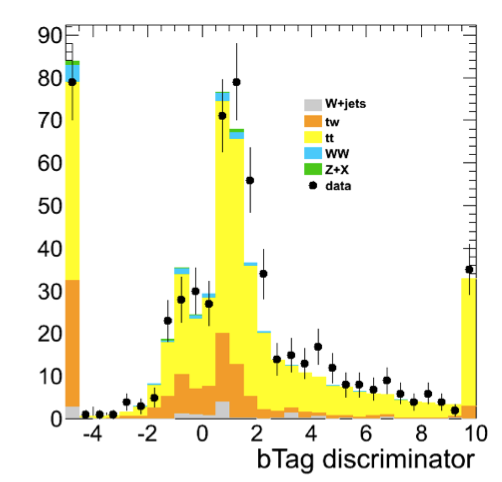
\includegraphics[width=0.3\linewidth]{figures/jetLowBtag_denum_dr.png} 
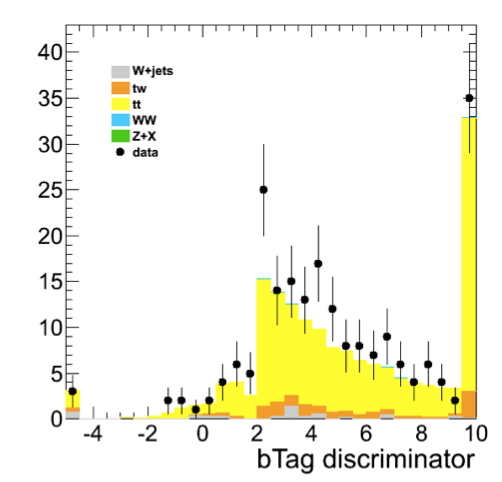
\includegraphics[width=0.3\linewidth]{figures/jetLowBtag_num_dr.png}
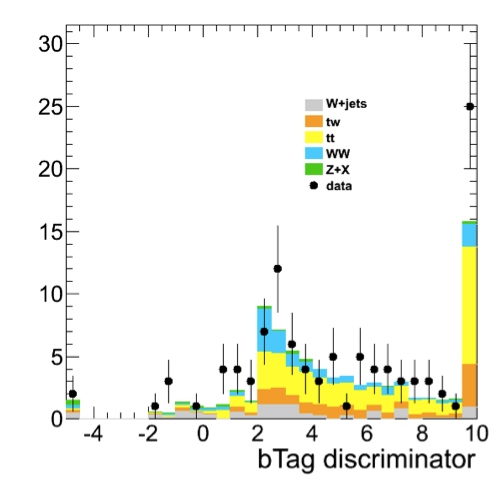
\includegraphics[width=0.3\linewidth]{figures/jetLowBtag_topTag_dr.png}
\caption{\label{fig:jetLowBtag}\protect b-tag discrimiator distribution for 
the jet with $p_T<30$ GeV and the highest b-tag discriminator in the 1-Jet (denumerator, left and numerator, center) 
and 0-Jet bins control region (right).}
\end{center}
\end{figure}
